\documentclass[crop,tikz]{standalone}
\usetikzlibrary{backgrounds}
\colorlet{blue}{cyan}
\tikzset{
  inverted/.style = {
    color=white,
    background rectangle/.style={fill},
    show background rectangle
  }
}

\usepackage{pgfplots}
\tikzset{>=latex}
\colorlet{green}{green}

\pgfplotsset{
  inverted/.style = {
    every axis legend/.append style={
      draw=white,
      fill=black,
      text=white
    }
  },
  every non boxed x axis/.append style={
    axis line style={-latex}
  },
  every non boxed y axis/.append style={
    axis line style={-latex}
  }
}

\newcommand{\axisstyle}{%
  thick,
  width=8cm,
  height=2.5cm,
  domain=0:10,
  samples=50,
  axis y line=middle,
  axis x line=middle,
  axis line style={draw=none},
  xlabel style={right},
  ylabel style={left},
  xmin=0, xmax=10,
  xticklabels={\empty},
  yticklabels={\empty},
  tick style={draw=none},
  samples=100,
  clip=false,%
}

\newcommand{\yshift}{-1.5cm}

\begin{document}
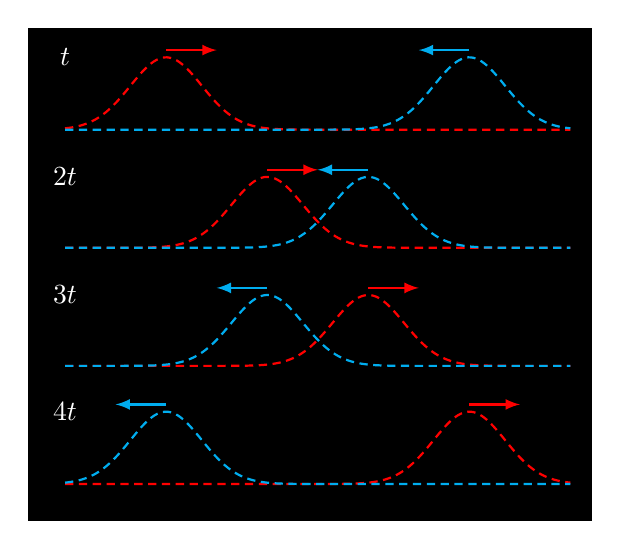
\begin{tikzpicture}[inverted,inverted]
\begin{axis}[inverted,
  \axisstyle
  ]
  \addplot[black,smooth] { exp(-(x-2)^2) + exp(-(x-8)^2) };
  \addplot[red  ,smooth, densely dashed] { exp(-(x-2)^2) };
  \addplot[blue ,smooth, densely dashed] { exp(-(x-8)^2) };
  \node at (axis cs: 0,1) {$t$};
  \draw[red ,->] (axis cs: 2,1.1) -- (axis cs: 3,1.1);
  \draw[blue,->] (axis cs: 8,1.1) -- (axis cs: 7,1.1);
\end{axis}
%
\begin{axis}[inverted,
  \axisstyle
  at={(0,\yshift)},
  ]
  \addplot[black,smooth] { exp(-(x-4)^2) + exp(-(x-6)^2) };
  \addplot[red ,smooth, densely dashed] { exp(-(x-4)^2) };
  \addplot[blue,smooth, densely dashed] { exp(-(x-6)^2) };
  \node at (axis cs: 0,1) {$2t$};
  \draw[red ,->] (axis cs: 4,1.1) -- (axis cs: 5,1.1);
  \draw[blue,->] (axis cs: 6,1.1) -- (axis cs: 5,1.1);
\end{axis}
%
\begin{axis}[inverted,
  \axisstyle
  at={(0,2*\yshift)},
  ]
  \addplot[black,smooth] { exp(-(x-6)^2) + exp(-(x-4)^2) };
  \addplot[red ,smooth, densely dashed] { exp(-(x-6)^2) };
  \addplot[blue,smooth, densely dashed] { exp(-(x-4)^2) };
  \node at (axis cs: 0,1) {$3t$};
  \draw[red ,->] (axis cs: 6,1.1) -- (axis cs: 7,1.1);
  \draw[blue,->] (axis cs: 4,1.1) -- (axis cs: 3,1.1);
\end{axis}
%
\begin{axis}[inverted,
  \axisstyle
  at={(0,3*\yshift)},
  ]
  \addplot[black,smooth] { exp(-(x-8)^2) + exp(-(x-2)^2) };
  \addplot[red ,smooth, densely dashed] { exp(-(x-8)^2) };
  \addplot[blue,smooth, densely dashed] { exp(-(x-2)^2) };
  \node at (axis cs: 0,1) {$4t$};
  \draw[red ,->] (axis cs: 8,1.1) -- (axis cs: 9,1.1);
  \draw[blue,->] (axis cs: 2,1.1) -- (axis cs: 1,1.1);
\end{axis}
\end{tikzpicture}
\end{document}
